\documentclass[9pt]{beamer}

\usetheme{Warsaw}
\usepackage[utf8]{inputenc}
\usepackage[spanish]{babel}
\usepackage{graphicx}
\usepackage{listings}
\usepackage{color}

\lstset{
  basicstyle=\tiny,
  commentstyle=\color{blue},
  keywordstyle=\color{red},
  language=Ruby
}

\AtBeginSection[]{
  \begin{frame}
    \tableofcontents[currentsection]
  \end{frame}
}

\AtBeginSubsection[]{
  \begin{frame}
    \tableofcontents[currentsection, currentsubsection]
  \end{frame}
}

\title{De por qué ED debió migrar a la web}
\subtitle{Ventajas de usar Frameworks y herramientas web para distribuir
          soluciones de desarrollo}
\author{Carlos Ledezma}
\institute{Akdemia}
\date{15/05/2014}

\begin{document}
  \frame{\titlepage}

  \frame{\tableofcontents}

  \section{Acerca de mí}
    \begin{frame}{Acerca de mí}
  \begin{itemize}
    \item ¿Por qué les hablo acerca de mí? \pause
    \item ¿Dónde trabajo?

      \vspace{0.25cm}
      \begin{center}
        
\includegraphics[scale=0.2]{img/akdemia} \pause
      \end{center}
    \item ¿De dónde vengo?

    \begin{center}
      \begin{tabular}{c c c}
        
\includegraphics[scale=0.2]{img/usb} &
        
\includegraphics[scale=0.2]{img/kth} &
        
\includegraphics[scale=0.2]{img/airbus} \
      \end{tabular}
    \end{center}
  \end{itemize}
\end{frame}


  \section{La historia de ED}
    \subsection{Presentación de ED}
  \begin{frame}{Él es ED}
  \begin{tabular}{l l}
    \parbox{0.5\textwidth}{
      \begin{itemize}
        \item Recién graduado.
        \item Inteligente.
        \item Emprendedor.
        \item Le gustan los retos.
        \item Poca experiencia laboral.
        \item Sólo código universitario.
        \item Muchas dudas.
      \end{itemize}
    } &
    \raisebox{-0.5\totalheight}{
\includegraphics[scale=0.5]{img/hello_ed}} \\
  \end{tabular}
\end{frame}

\begin{frame}{ED tiene una idea}
  \begin{tabular}{r l}
    \raisebox{-0.5\totalheight}{
\includegraphics[scale=0.3]{img/ed_and_client}} &
    \parbox{0.5\textwidth}{
      \begin{itemize}
        \item Encontró un nicho no explotado.
        \item Tiene un cliente potencial, C.
        \item Le desarrollará P a C.
      \end{itemize}
    } \\
  \end{tabular} \pause
  \begin{center}
    \textbf{EMPIEZA EL DESARROLLO!!!}
  \end{center}
\end{frame}

\subsection{El proceso de desarrollo}
  \begin{frame}{Escoger un lenguaje}
  \begin{center}
    \begin{tabular}{c c c c}
      
\includegraphics[scale=0.1]{img/cpp} & \pause
      
\includegraphics[scale=0.15]{img/java} & \pause
      
\includegraphics[scale=0.15]{img/haskell} & \pause
      
\includegraphics[scale=0.1]{img/erlang} \\

      
\includegraphics[scale=0.05]{img/matlab} &
      
\includegraphics[scale=0.05]{img/pascal} &
      
\includegraphics[scale=0.15]{img/prolog} &
      
\includegraphics[scale=0.1]{img/smalltalk} \\
    \end{tabular}

    
\includegraphics[scale=0.3]{img/choose_ed}
  \end{center}
\end{frame}

\begin{frame}{Comunicación con la base de datos}
  \begin{itemize}
    \item sqlapi \pause $\rightarrow$ GCC. \pause
    \item MySQL connector \pause $\rightarrow$ ED quiere PostgreSQL. \pause
    \item libodbc \pause $\rightarrow$ Aún en desarrollo. \pause
    \item libpqxx.
  \end{itemize}
\end{frame}

\begin{frame}{Interfaz gráfica}
  \begin{itemize}
    \item Qt.
    \item gtkmm.
    \item wxWidgets.
    \item FLTK.
  \end{itemize}
\end{frame}

\begin{frame}{Diseño estructural}
  Implementar diseño en capas:
  \begin{itemize}
    \item Modelo $\rightarrow$ Encapsular llamadas a DB.
    \item Controlador $\rightarrow$ Crear puentes de comunicación.
    \item Vista $\rightarrow$ Comunicar con librería gráfica.
    \item Debe haber total separación.
  \end{itemize}

  \begin{center}
    
\includegraphics[scale=0.5]{img/ed_realization}
  \end{center}
\end{frame}

\subsection{La entrega de la solución}
  \begin{frame}{Colocando todo en el pendrive}
  ED compila su producto:
  \begin{itemize}
    \item ¿Arquitectura correcta?
    \item Hacer instalador.
    \item ¿Requerimientos en el cliente?
    \begin{itemize}
      \item Manejador de base de datos.
      \item Librerías gráficas.
      \item ¿Documentados requerimientos?
      \item Lidiar con máquinas diferentes.
    \end{itemize}
  \end{itemize}
\end{frame}

\subsection{La etapa de soporte}
  \begin{frame}{Los primeros errores}
  \begin{tabular}{l c}
    \raisebox{-0.5\totalheight}{
\includegraphics[scale=0.5]{img/ed_q_a}} &
    \parbox{0.5\textwidth}{
      \begin{itemize}
        \item Primer intento $\rightarrow$ teléfono. \pause
        \item \textbf{JA} \pause
        \item ED debe buscar sus bitácoras.
      \end{itemize}
    } \\
  \end{tabular}
\end{frame}

\begin{frame}{Hora de analizar}
  \begin{center}
    
\includegraphics[scale=0.1]{img/ed_inquiry}
  \end{center} \pause
  Posibles errores:
  \begin{itemize}
    \item Librería de comunicación. \pause
    \item Manejo de memoria. \pause
    \item Particulares de la arquitectura.
  \end{itemize}
\end{frame}

\begin{frame}{A solucionar los problemas}
  \begin{tabular}{l l}
    \parbox{0.5\textwidth}{
      \begin{itemize}
        \item Pasar un par de semanas corrigiendo.
        \item Recompilar.
        \item Crear instalador.
        \item Llevaro al cliente.
      \end{itemize}
    } &
    \raisebox{-0,5\totalheight}{
\includegraphics[scale=0.1]{img/ed_solving}} \\
  \end{tabular} \pause
  \begin{center}
    Proceso se repite con cada error \pause $\rightarrow$ Soluciones lentas
  \end{center}
\end{frame}

\subsection{La conclusión evidente}
  \begin{frame}{ED pierde a su cliente}
  \begin{center}
    
\includegraphics[scale=0.5]{img/ed_crushed}
  \end{center}
\end{frame}



  \section{Ayudando a ED}
    \subsection{Sugerencia y presentación de la herramienta}
  \begin{frame}{Salvemos a ED usando RoR}
  ¿Qué es Ruby on Rails?
  \begin{tabular}{l c}
    \parbox{0.5\textwidth}{
      \begin{itemize}
        \item Framework de desarrollo web.
        \item Basado en Ruby.
        \item M.V.C.
        \item CoC
        \item Incluye todos los procesos del desarrollo web.
        \item Apoyado por gemas.
      \end{itemize}
    } &
    \raisebox{-0.5\totalheight}{
\includegraphics[scale=0.2]{img/ror}}
  \end{tabular}
\end{frame}

\begin{frame}{El modelo M.V.C. de RoR}
  \centering
  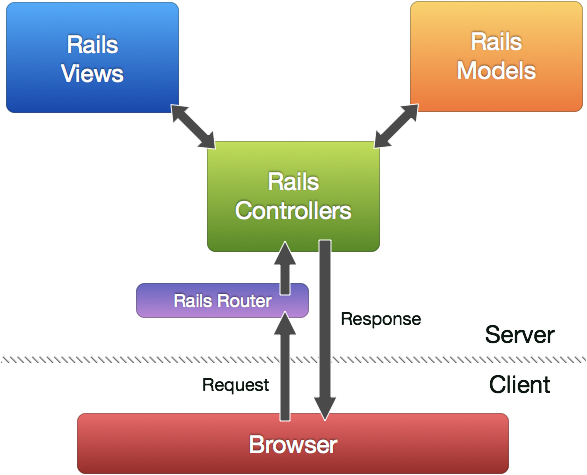
\includegraphics[scale=0.3]{img/railsmvc}
\end{frame}

\begin{frame}[fragile]{Convenciones sobre la configuración}
  Lo básico:

  \pause

  \begin{tabular}{l l}
    \parbox{0.5\textwidth}{
      app/models/:
      \begin{itemize}
        \item ActiveRecord::Base.
        \item Clases $\leftrightarrow$ Tablas.
        \item Infinidad de métodos predefinidos.
      \end{itemize}
    } \pause &
    \begin{lstlisting}
# app/models/user.rb
class User < ActiveRecord::Base
  belongs_to :company # modelo Company
  has_many :associates # modelo Associate
  has_one :session # modelo Sessions

  ...
end
    \end{lstlisting} \pause \\

    \parbox{0.5\textwidth}{
      app/controllers/:
      \begin{itemize}
        \item ActionController::Base.
        \item Manejan la lógica.
        \item Reciben peticiones.
      \end{itemize}
    } \pause &
    \begin{lstlisting}
# app/controllers/users_controller.rb
class UsersController < ActionController::Base
  def index
    @users = User.where( ... )
  end

  ...
end
    \end{lstlisting} \pause \\

    \parbox{0.5\textwidth}{
      app/views:
      \begin{itemize}
        \item Archivos .erb.
        \item Contienen las interfaces.
        \item HTML, Haml.
      \end{itemize}
    } \pause &
    \begin{lstlisting}[language=HTML]
<!-- app/views/users/index.html.erb -->
...
<% @users.each do |user| % >
  <p> <% = user.name % > </p>
<% end % >
...
    \end{lstlisting}
  \end{tabular}
\end{frame}

\begin{frame}{Apoyo de las gemas (demos)}
  \begin{tabular}{l l}
    \raisebox{-0.5\totalheight}{
\includegraphics[scale=0.4]{img/rails_gems}} &
    \pause 

    \parbox{0.5\textwidth}{
      \begin{itemize}
        \item Squeel $\rightarrow$ Mejor SQL. \pause
        \item Pry $\rightarrow$ Depuración. \pause
        \item CanCan $\rightarrow$ Autorización. \pause
        \item Authlogic $\rightarrow$ Autenticación. \pause
        \item simple\_form, prawn, nested\_form, spreadsheet, haml, zeus,
        jquery\_rails...
      \end{itemize}
    }
  \end{tabular}

  \begin{center}
    \textbf{INVIERTE TU TIEMPO EN TU PROYECTO}
  \end{center}
\end{frame}


\begin{frame}{Ahora, volvamos con ED}
  \centering
  
\includegraphics[scale=0.8]{img/hello_ed}
\end{frame}

\subsection{El proceso de desarrollo}
  \begin{frame}{Todo es tan fácil en RoR}
  \begin{tabular}{c l}
    \raisebox{-0.5\totalheight}
             {
\includegraphics[scale=0.3]{img/ed_building_ror}} &

    \pause

    \parbox{0.5\textwidth}{
      \begin{itemize}
        \item Lenguaje $\rightarrow$ Ruby + RoR. \pause
        \item Comunicación con B.D. $\rightarrow$ pg + database.yml. \pause
        \item Interfaz $\rightarrow$ HTML + CSS. \pause
        \item Estructura $\rightarrow$ MVC.
      \end{itemize}
    } \\
  \end{tabular}
\end{frame}

\subsection{La entrega de la solución}
  \begin{frame}{¿En un pendrive?}
  \begin{tabular}{l c}
    \raisebox{-0.5\totalheight}{
\includegraphics[scale=0.3]{img/ed_amazed}} &
    \pause

    \parbox{0.5\textwidth}{
      \begin{itemize}
       \item ¿Compilación? $\rightarrow$ Ruby interpretado. \pause
       \item ¿Instalador? $\rightarrow$ Entregar vía web:

       \begin{itemize}
        \item Heroku.
        \item Amazon Web Services.
        \item ...
       \end{itemize} \pause
        
        \item Requerimientos del cliente $\rightarrow$ Un navegador + intenet.
      \end{itemize}
    } \\
  \end{tabular}
\end{frame}

\subsection{La etapa de soporte}
\subsection{Algunos extras}
\subsection{La conclusión evidente}


  \section{Despedida y preguntas}
    \begin{frame}{Conclusiones}
  \centering
  \textbf{CONCLUSIONES}
\end{frame}

\begin{frame}{Preguntas}
  \centering
  
\includegraphics[scale=0.2]{img/ed_inquiry}
\end{frame}

\end{document}
